\chapter[Descripción metodológica\dots]{Descripción metodológica del trabajo \sectionmark{Metodología}}
\sectionmark{Metodología}

El proceso de trabajo llevado a cabo para el presente proyecto, así como sus tiempos de planificación y ejecución, se exponen aquí desde dos perspectivas: la del proyecto global desde su concepción (investigación, contactos, visitas al GME, etc.), y la del desarrollo del software en sí, que lleva su propio tiempo y calendario. 

\section[El proyecto en su conjunto]{El proyecto en su conjunto \sectionmark{El proyecto\dots}}
\sectionmark{El proyecto\dots}

Una vez definida la idea general del proyecto, se procedió a dar lo siguientes pasos:

\subsection{Toma de contacto con los responsables del GME en la universidad de Castilla--La Mancha. }

Este era el primer paso a dar tanto desde el punto de vista cronológico como lógico. Las personas con las que puede entrevistar entre octubre y noviembre fueron precisamente las encargadas actualmente del Gabinete, Sylvia Molina Muro\footnote{Prof. contratado doctor (UCLM). Investigador principal del grupo I+D+I <<Fuzzy Gab 4>>, encargado de la recuperación y dinamización de los fondos GME en el ITCT (CUenca--UCLM).} y Julio Sanz Vázquez, compositor y técnico del Gabinete. Ambos acogieron con gran entusiasmo el proyecto y pude acceder con ellos a las instalaciones de estudio actual en varias ocasiones.

\subsection{Investigación sobre los sintetizadores de EMS}

No se han encontrado manuales de usuario del Synthi 100. Sí que existe un <<manual de servicio>>, cuya finalidad es la de ofrecer datos técnicos para ingenieros en electrónica, no una guía de uso para músicos o artistas sonoros. Sin embargo, EMS sí que publicó manuales de usuario para modelos de sintetizadores más <<domésticos>>, como el Synthi AKS\citeyear{SynthiAKS_brochure}, Synthi CVS3\citeyear{SynthiVCS3_brochure}. Existen muchas similitudes entre estos sintetizadores y el Synthi 100, a pesar de las diferencias de tamaño. En todos los casos el sistema de conexiones es el de una matriz, por lo que la filosofía de funcionamiento es muy similar entre ellos. El uso de emuladores ya implementados fue una gran ayuda para comprender el funcionamiento de muchos módulos, más allá de la intuición y de la relación con otros la sección sintetizadores documentados\footnote{Sobre los plugins y diversos emuladores, véase la sección \ref*{sec:plugins} en la página \pageref{sec:plugins}}.

\subsection{Inicio del desarrollo de la \textit{app}}

El desarrollo de la aplicación de software, \appName, objeto de esta memoria, no podía ser pospuesto al momento de tener toda la información posible acerca del sintetizador, así como el comportamiento particular del Synthi 100 del GME. Al contrario, era imprescindible plantear desde el inicio la estructura de su código, el estilo de programación, etc. de modo que la implementación de los diversos módulos del sintetizador no estuviera fuertemente condicionada por la arquitectura general del programa. La elaboración del programa en SuperCollider fue siempre paralela a la de toda investigación y recogida de información del Synthi 100 o del GME.

\subsection{Fotografiado exhaustivo del Synthi 100 en el GME}

Esta tarea fue crucial para conocer al detalle la interfaz del sintetizador, por una parte, y como base de la interfaz gráfica del programa, por otra. Esta sesión tuvo lugar a mediados de diciembre. Había prevista una nueva sesión para obtener fotografías de mayor calidad en el mes de abril que, lógicamente, no pudo llevarse a cabo. Estas nuevas fotografías, que serán realizadas en otro momento en el futuro, estarán destinadas a la interfáz gráfica de usuario.

\subsection{Sesiones de pruebas y testeos en el GME}

En enero de 2020 comenzó a estar operativo el Synthi 100 en su proceso de restauración. En ese mismo mes pude experimentar con el comportamiento de varios de sus módulos (fig. \ref{fig:Synthi_Synthi}). Es evidente que este trabajo de campo con el sintetizador se puede traducir en una ingente cantidad de horas de experimentación y registro de materiales sonoros que exceden los límites de este trabajo. En todo caso, se trata de un trabajo que es imprescindible para una futura evolución de la aplicación.

\begin{figure}
	\centering
	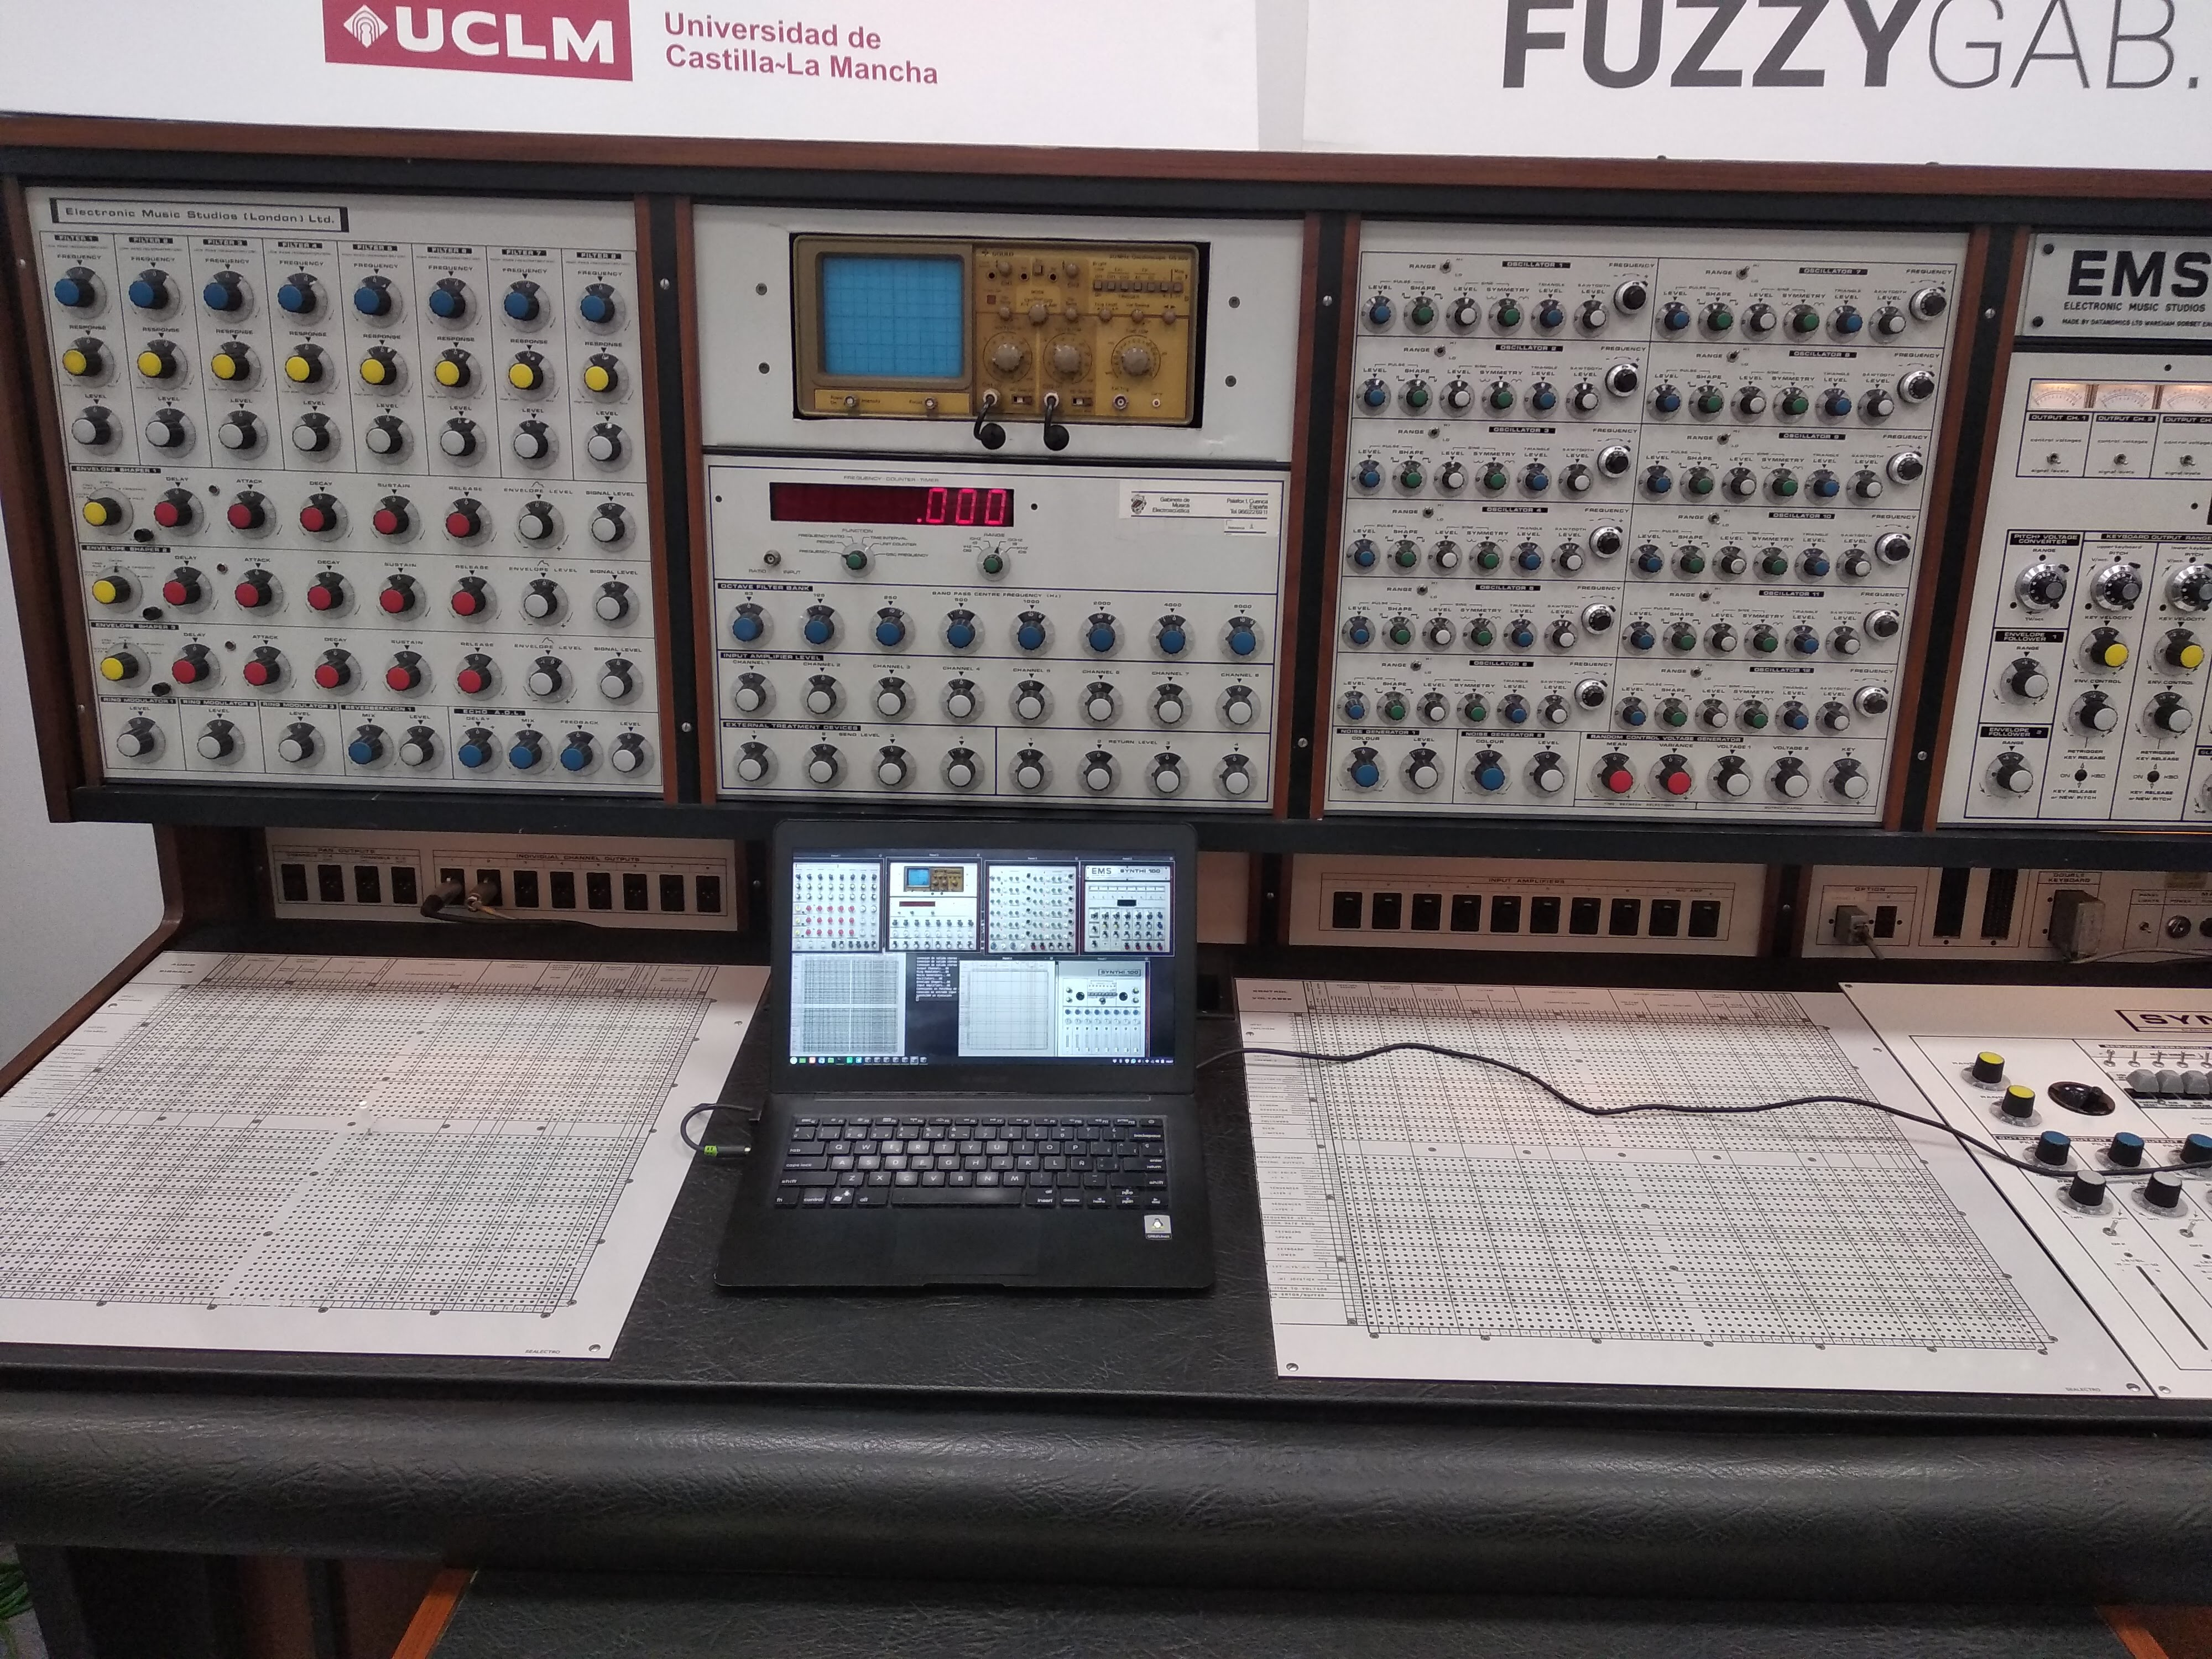
\includegraphics[width=0.7\textwidth]{Synthi_Synthi}
	\caption[Aplicación \appName~ejecutándose junto al Synthi 100 en el GME]{Aplicación \appName~ejecutándose junto al Synthi 100 en el GME, realizando testeos y pruebas en los diferentes módulos implementados.}
	\label{fig:Synthi_Synthi}
\end{figure}

\section[La programación\dots]{La programación de \appName \sectionmark{La programación\dots}}
\sectionmark{La programación\dots}

Todo desarrollo de software requiere de un gran esfuerzo organizativo así como una buena estructuración de las diversas etapas. Consumir una etapa antes de tiempo puede provocar problemas irresolubles en el futuro. Desde el inicio, el código ha estado bajo el control de versiones \textit{Git}, y alojado en la plataforma \textit{Github}\footnote{En el momento de la escritura de esta memoria, el repositorio donde se encuntra todo el código es \href{https://github.com/mesjetiu/SynthiGME}{\texttt{https://github.com/mesjetiu/SynthiGME}}}. Este sistema permite registrar todos los cambios de código realizados momento a momento, con descripciones de las mismas. Además, permite el versionado y es imprescindible para poder ser instalado y utilizado como un paquete, de modo que el usuario no necesita trabajar directamente con el código del programa para poder ejecutarlo.

Las diversas etapas de desarrollo pueden observarse directamente en el repositorio en \textit{Github}, y pueden resumirse en los siguientes puntos:

\begin{description} 
	\item[Establecimiento de una estructura global del código] Se trata de un proceso iterativo, en el que es necesario realizar toda una serie de pruebas de concepto. El resultado de dichas pruebas van aportando información muy valiosa a la hora de tomar decisiones que quedarán en la estructura de la aplicación. Una mala arquitectura y jerarquía en las clases, sus métodos, su interfaz, etc., pueden acarrear problemas en el futuro, cuya resolución es muy costosa en cuanto a tiempo de trabajo. El primer mes de trabajo fue esencial para la continuación exitosa hasta el día de hoy.
	
	\item[Implementación de una interfaz gráfica externa] Los primeros elementos de la aplicación no podían manejarse desde ninguna interfaz gráfica. Todo se debía de manejar con código (algo natural, por otra parte, en SuperCollider). En un primer momento se prentendía separar completamente la interfaz gráfica del motor del sonido, de modo que dicha interfaz pudiera ser programada en cualquier lenguaje y en cualquier plataforma y su comunicación con el motor se realizaría íntegramente con mensajes OSC\footnote{Véase la sección \ref{sec:osc} dedicada al protocolo \textit{OSC} (pág. \pageref{sec:osc}).}. Una vez implementado este protocolo, incluso diseñada en parte una interfaz para móvil y tablet, se vio oportuno que la aplicación tuviera una interfaz gráfica en el propio ordenador, por defecto.
	
	\item[Implementación de la interfaz gráfica en SuperCollider] Hasta enero de 2020 aproximadamente, todo el código estaba dirigido a una interfaz OSC, arriba descrita, y ciertos módulos de prueba. La creación de una interfaz gráfica para el propio ordenador fue un punto de inflexión en el desarrollo de la aplicación. El Synthi 100 es demasiado grande como para ser contenido en pantallas móviles, y poco práctico si se plantea como diversas páginas de una aplicación móvil. La pantalla del ordenador permitía ver todos los módulos de un solo vistazo. Su inmediated, por otra parte, agilizó mucho el desarrollo de la aplicación. El lenguaje de programación, por otra parte, es el mismo que el del resto de los módulos, \textit{sclang}, y, en beneficio de un aspecto más realista, fue posible usar fotografías del Synthi 100 para realizar su diseño.
	
	\item[Implementacion del resto de módulos] Una vez que interfaz gráfica y módulos estaban al mismo nivel de desarrollo, la evolución de ambos caminó a la par hasta hoy. Módulo a módulo fue siendo implementado y testeado en su conjunto. Con cierta frecuencia aparecían \textit{bugs} por suerte corregidos exitosamente. Esta etapa es la que llega hasta el presente y se proyecta hacia el futuro. El esqueleto de la app está terminado, con una gran parte de sus módulos implementados y funcionando de forma lógica e intercomunicada. Desde esta misma etapa, la aplicación ya pudo ser usada de forma funcional.
\end{description}




